\documentclass[10pt,a4paper]{report}

\usepackage[a4paper,top=3cm,bottom=3cm,left=2cm,right=2cm]{geometry}
%bindingoffset=5mm

% per la codifica dei font
\usepackage[latin1]{inputenc}
\usepackage[T1]{fontenc}
\usepackage[italian]{babel}

% per l'interlinea
\usepackage{setspace}

% per le immagini
\usepackage[dvips]{graphicx}

% per la matematica
\usepackage{amsmath,amssymb,euler,mathtools}

\DeclarePairedDelimiter{\abs}{\lvert}{\rvert}
\DeclarePairedDelimiter{\norma}{\lVert}{\rVert}

% per l'inserimento del codice nel testo
\usepackage{listings}
\lstset{language=python, basicstyle=\small\ttfamily}
\lstnewenvironment{codice}{\lstset{language=python, basicstyle=\small\ttfamily, showstringspaces=false}}{}

% per gli url nella bibliografia
\usepackage{url}

% per le didascalie
\usepackage[hang,small,bf]{caption}

\usepackage{fancyhdr}
\fancyhead[R]{}

% per l'inserimento e l'affiancamento delle immagini
\usepackage[usenames]{color}
\usepackage{subfig}

% per gli elenchi 
\usepackage{enumitem}

\usepackage{booktabs}

\usepackage{array} 

\usepackage{float}

\begin{document}
\pagestyle{empty}

\begin{center}
  %%% Logo
  \begin{figure}
    \centering
    
\includegraphics[width=0.5\textwidth]{logo}
    \vspace{1.5 cm}
  \end{figure}
  %%%

  %%% Facoltà, Corso di studi
  \Large
  {\fontfamily{pag} \selectfont{\scshape Dipartimento di Matematica e Fisica\\}}
  \vspace{0.1 cm}
  Corso di Studi Magistrale in Scienze Computazionali\\
  \vspace{0.1 cm}
  \large
  {\fontfamily{pag} \selectfont{\scshape Insegnamento di Calcolo parallelo e distribuito\\}}
  %%%

  \vspace{3.5 cm}

  %%% TITOLO
  \huge
  \selectfont{\bfseries{\textsf{MODULO \texttt{larcc}\\TRADUZIONE IN JULIA\\E PARALLELIZZAZIONE}}}
  %%%

  \vspace{3.5 cm}

  \large
  \begin{tabular}[t]{@{}l}
%    {\fontfamily{pag} \selectfont {\scshape Relatore:}}\\
    {\fontfamily{pag} {Prof. Alberto Paoluzzi}}\\
  \end{tabular}
  \hfill
  \begin{tabular}[t]{@{}r}
%    {\fontfamily{pag} \selectfont {\scshape Presentata da:}}\\
    {\fontfamily{pag} {Sarah Tofoni}}\\
    {\fontfamily{pag} {Martina Trani}}\\
  \end{tabular}

  \vspace{3.5 cm}

  %%% Anno Accademico
%  {\fontfamily{pag} \selectfont {\scshape Sessione invernale\\}}
%  \vspace{0.1 cm}
  {\fontfamily{pag} \selectfont {\scshape A.A. 2017-2018}}
  %%%   
\end{center}


\pagestyle{empty}
\pagenumbering{arabic}
\tableofcontents
\pagestyle{fancy}
\pagenumbering{arabic}
\singlespacing

\chapter{Introduzione}

\section{Modulo \texttt{larcc}}
Nel modulo \texttt{larcc} vengono utilizzate delle rappresentazioni topologiche basilari, che includono alcuni comuni formati per le matrici sparse:
\begin{enumerate}
 \item CSR, \emph{Compressed Sparse Row}
 \item CSC, \emph{Compressed Sparse Column}
 \item COO, \emph{Coordinate Representation}
 \item BRC, \emph{Binary Row Compressed}
\end{enumerate}

\subsection{CSR (Compressed Sparse Row)}
Il formato \emph{Compressed Sparse Row} (CSR) memorizza una matrice $M$ di dimensione $m x n$ sparsa in forma di riga, utilizzando tre matrici 
unidimensionali $A$, $IA$, $JA$.\\
L'array $A$ contiene tutte i valori di $M$ diversi da zero, in ordine da sinistra a destra dall'alto verso il basso.\\
L'array $IA$ � di lunghezza $m + 1$, definito ricorsivamente nel modo seguente:
\begin{itemize}
 \item $IA_0 = 0$
 \item $IA_i = IA_{i - 1}$ + numero di elementi diversi da zero nella riga $i-1$ della matrice originale
\end{itemize}
Il terzo array, $JA$, contiene l'indice di colonna in $M$ di ciascun elemento di $A$. 

\subsection{CSC (Compressed Sparse Column)}
Il formato \emph{Compressed Sparse Column} (CSC) � simile a quello precedente, a eccezione del fatto che i valori vengono letti prima per colonna, 
viene memorizzato un indice di riga per ogni valore e vengono memorizzati i puntatori di colonna. 

\subsection{COO (Coordinate Representation)}
Il formato \emph{Coordinate Representation} (COO) memorizza una lista di tuple \emph{riga, colonna, valore}. Idealmente, le voci sono ordinate prima 
per indice di riga e poi per indice di colonna, per migliorare i tempi di accesso casuale.

\subsection{BRC (Binary Row Compressed)}
Il formato \emph{Binary Row Compressed} (BRC), nell'infrastruttura \texttt{larcc}, � il formato standard di matrice, utilizzato per rappresentare una 
matrice binaria solitamente sparsa.\\
Tale rappresentazione consiste in un array di array di interi, in cui gli array componenti non hanno necessariamente la stessa dimensione. Ogni array 
componente, corrispondente a una riga della matrice, contiene gli indici delle colonne in corrispondenza dei quali � memorizzato un $1$, mentre non 
viene tenuta traccia di eventuali zeri.

\section{Funzioni selezionate}
La scelta delle funzioni di cui realizzare la traduzione sequenziale da Python a Julia � stata effettuata in base alla frequenza con la quale le 
stesse venivano richiamate all'interno dei test del modulo. Di ognuna di queste funzioni selezionate, vengono riportati una breve descrizione del 
comportamento, il codice originario in Python, la relativa traduzione in Julia, la versione parallela e i tempi di esecuzione.

\vspace{1 cm}

\begin{tabular}{p{4.8 cm} p{4.8 cm} p{4.8 cm}}
\toprule
\textbf{API}			& \textbf{Locali} 		& \textbf{Funzioni esterne} 	\\
\midrule
\texttt{csrCreate}		&				& 				\\
\texttt{brc2Coo}		&				& 				\\
\texttt{coo2Csr}		&				& 				\\
\texttt{triples2mat}		&				& 				\\
\texttt{csr2DenseMatrix}	&				& 				\\
\texttt{csrGetNumberOfRows}	&				& 				\\
\texttt{csrGetNumberOfColumns}	&				& 				\\
\texttt{larModelNumbering}	& \texttt{larModelNumbering0} 	& \texttt{cellNumbering}	\\
\texttt{larFacets}		&				& 				\\
\texttt{setup}			&				& 				\\
\texttt{larCellAdjacencies}	&				& 				\\
\texttt{matrixProduct}		&				& 				\\
\texttt{csrTranspose}		&				& 				\\
\texttt{csrPredFilter}		&				& 				\\
\texttt{mkSignedEdges}		& 				& 				\\
\bottomrule
\end{tabular}

\vspace{1 cm}

\section{Grafico delle dipendenze tra funzioni}

\begin{figure}[H]
  \centering 
  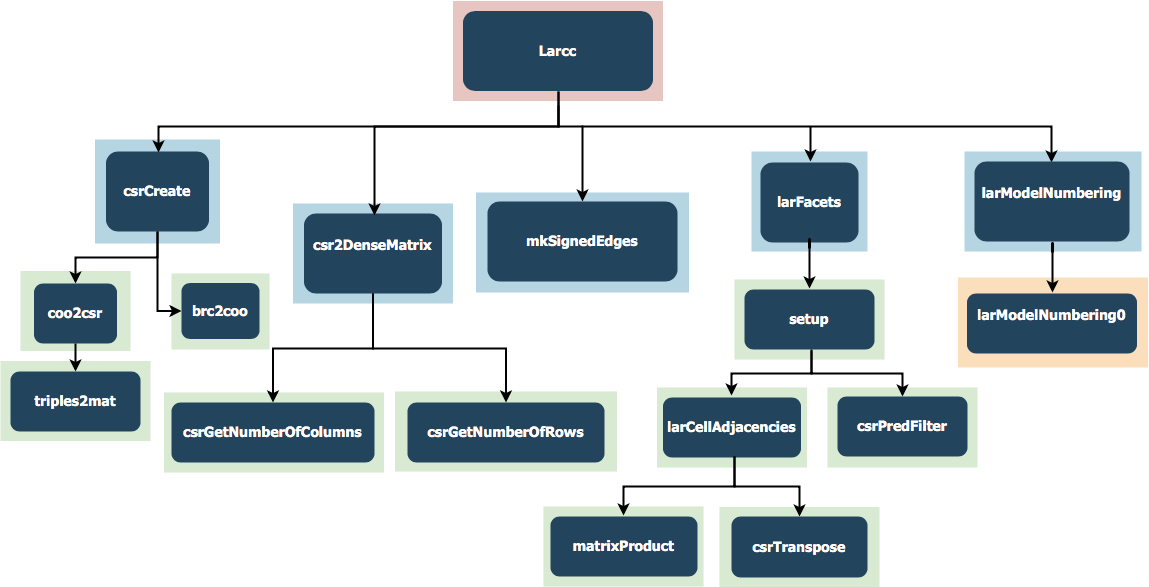
\includegraphics[width=1\columnwidth]{immagini/Larcc}
\end{figure}

\vspace{1 cm}

\section{Tempi di esecuzione}
Per calcolare i tempi di esecuzione delle funzioni, sia in versione seriale sia parallelizzata, sono state utilizzate la macro \texttt{@elapsed} e la 
macro \texttt{@timev} (versione \emph{verbose} della macro \texttt{@time}). La prima resituisce soltanto il tempo in secondi, la seconda restituisce 
anche la quantit� di memoria allocata. \\

\noindent Dal momento che alla prima chiamata di \texttt{@elapsed f(args)} o \texttt{@timev f(args)} la funzione \texttt{f} deve essere compilata 
prima che eseguita, il primo utilizzo delle macro non deve essere considerato, perch� il tempo di esecuzione sar� sicuramente peggiore del normale.

\singlespacing

\chapter{Implementazione}

\section{csrCreate, brc2Coo, coo2Csr, triples2mat}

\texttt{csrCreate}: effettua la conversione dal formato BRC (Binary Row Compressed) al formato CSR (Compressed Sparse Row), utilizzando due modi 
differenti a seconda se la dimensione della matrice � sconosciuta (\texttt{shape=(0,0)}) o no. \\
% Conversion from BRC to CSR format. The transformation from BRC to CSR format is implemented slightly differently, according to the fact that the 
% matrix dimension is either unknown (shape=(0,0)) or known

\noindent \texttt{brc2Coo}: trasforma una matrice in rappresentazione BRC in una lista di triple (\emph{riga, colonna, 1}), ordinate per riga. \\
% From triples to scipy.sparse The function brc2Coo transforms a BRC representation in a list of triples (row, column, 1) ordered by row.

\noindent \texttt{coo2Csr}: effettua la conversione dalle triple al formato CSR. \\
%The conversion from triples to csr format is provided below.

\noindent \texttt{triples2mat}: realizza la trasformazione della matrice in formato \emph{sparso}, data come lista di triple (\emph{riga, colonna, 
valore}) di elementi non nulli, nel formato \texttt{scipy.sparse} corrispondente al parametro \texttt{shape} in ingresso, settato di default a 
\texttt{csr}, il formato standard dell'infrastruttura \texttt{larcc}.
% Conversion to csr format Then we give the function triples2mat to make the transformation from the sparse matrix, given as a list of triples 
% row,column,value (non-zero elements), to the scipy.sparse format corresponding to the shape parameter, set by default to "csr", that stands for 
% Compressed Sparse Row, the normal matrix format of the LARCC framework.

\subsection{Traduzione}

\textbf{Python}

\begin{codice}
def triples2mat(triples, shape = "csr"):
    n = len(triples)
    data = arange(n)
    ij = arange(2*n).reshape(2,n)
    for k, item in enumerate(triples):
	ij[0][k], ij[1][k], data[k] = item
    return scipy.sparse.coo_matrix((data,ij)).asformat(shape)
\end{codice}

\vspace{0.5 cm}

\begin{codice}
def brc2Coo(ListOfListOfInt):
    COOm = [[k,col,1] for k,row in enumerate(ListOfListOfInt) for col in row]
    return COOm
\end{codice}

\vspace{0.5 cm}

\begin{codice}
def coo2Csr(COOm):
    CSRm = triples2mat(COOm, "csr")
    return CSRm
\end{codice}
  
\vspace{0.5 cm}

\begin{codice}
def csrCreate(BRCmatrix, lenV = 0, shape = (0,0)):
    triples = brc2Coo(BRCmatrix)
    if shape == (0,0):
	CSRmatrix = coo2Csr(triples)
    else:
	CSRmatrix = scipy.sparse.csr_matrix(shape)
	for i,j,v in triples: 
	    CSRmatrix[i,j] = v
    return CSRmatrix
\end{codice}

\vspace{0.5 cm}

\noindent \textbf{Julia}

\begin{codice}
function triples2mat(triples, shape = "csr")
    n = length(triples)
    data = collect(1:n)
    i = collect(0:n-1)
    j = collect(n:2n-1)
    ij = [i,j]
    for e in enumerate(triples)
	k = e[1]
	ij[1][k] = triples[k][1]
	ij[2][k] = triples[k][2]
	data[k] = triples[k][3]
    end
    return ss.coo_matrix((data,ij))[:asformat](shape)
end
\end{codice}

\vspace{0.5 cm}

\begin{codice}
function brc2Coo(BRCmatrix)
    COOmatrix = vcat([[k-1,col,1] for (k,row) in enumerate(BRCmatrix) 
		for col in row])
    return COOmatrix
end
\end{codice} 

\vspace{0.5 cm}

\begin{codice}
function coo2Csr(COOmatrix)
    CSRmatrix = triples2mat(COOmatrix, "csr")
    return CSRmatrix
end
\end{codice}

\vspace{0.5 cm}

\begin{codice}
function csrCreate(BRCmatrix, lengthV = 0, shape = (0,0))
    triples = brc2Coo(BRCmatrix)
    if shape == (0,0)
	CSRmatrix = coo2Csr(triples)
    else
	CSRmatrix = ss.csr_matrix(shape)
	for (i,j,v) in triples
	    CSRmatrix[i,j] = v
	end
    end
    return CSRmatrix 
end 
\end{codice}

\vspace{0.5 cm}

\subsection{Versione parallela}

\begin{codice}
@everywhere function ptriples2mat(triples, shape = "csr")
    n = length(triples)
    data = collect(1:n)
    i = collect(0:n-1)
    j = collect(n:2n-1)
    ij = [i,j]
    @sync for e in enumerate(triples)
	k = e[1]
	ij[1][k] = triples[k][1]
	ij[2][k] = triples[k][2]
	data[k] = triples[k][3]
    end
    return ss.coo_matrix((data,ij))[:asformat](shape)
end
\end{codice}

\vspace{0.5 cm}

\begin{codice}
@everywhere function pbrc2Coo(BRCmatrix)
    COOmatrix = vcat([[k-1,col,1] for (k,row) in enumerate(BRCmatrix) 
		for col in row])
    return COOmatrix
end
\end{codice}

\vspace{0.5 cm}

\begin{codice}
@everywhere function pcoo2Csr(COOmatrix)
    CSRmatrix = ptriples2mat(COOmatrix, "csr")
    return CSRmatrix
end
\end{codice}

\vspace{0.5 cm}

\begin{codice}
@everywhere function pcsrCreate(BRCmatrix, lengthV = 0, shape = (0,0))
    triples = pbrc2Coo(BRCmatrix)
    if shape == (0,0)
	CSRmatrix = pcoo2Csr(triples)
    else
	CSRmatrix = ss.csr_matrix(shape)
	@sync for (i,j,v) in triples
	    CSRmatrix[i,j] = v
	end
    end
    return CSRmatrix 
end 
\end{codice}

\vspace{0.5 cm}

\subsection{Tempi di esecuzione}

\noindent \textbf{Seriale}

\begin{codice}
julia> @timev csrCreate(EV)
  0.001009 seconds (156 allocations: 8.359 KiB)
elapsed time (ns): 1009260
bytes allocated:   8560
pool allocs:       156
PyObject <9x6 sparse matrix of type '<type 'numpy.int64'>'
	with 18 stored elements in Compressed Sparse Row format>
\end{codice}

\vspace{0.5 cm}

\noindent \textbf{Parallela con lo stesso numero di processori}

\begin{codice}
julia> @timev pcsrCreate(EV)
  0.000569 seconds (156 allocations: 8.359 KiB)
elapsed time (ns): 569140
bytes allocated:   8560
pool allocs:       156
PyObject <9x6 sparse matrix of type '<type 'numpy.int64'>'
	with 18 stored elements in Compressed Sparse Row format
\end{codice}

\vspace{0.5 cm}

\pagebreak

\noindent \textbf{Parallela con l'aggiunta di 15 processori}

\begin{codice}
julia> @timev pcsrCreate(EV)
  0.002283 seconds (156 allocations: 8.359 KiB)
elapsed time (ns): 2282594
bytes allocated:   8560
pool allocs:       156
PyObject <9x6 sparse matrix of type '<type 'numpy.int64'>'
	with 18 stored elements in Compressed Sparse Row format>
\end{codice}


\section{csr2DenseMatrix, csrGetNumberOfRows, csrGetNumberOfColumns}

\texttt{csr2DenseMatrix}: il pacchetto \texttt{scipy} fornisce l'utile metodo \texttt{.todense()} allo scopo di trasformare ogni matrice nel formato 
\emph{sparso} nel corrispondente formato \emph{denso}. Per ragioni di generalit� e portabilit� � riportata la funzione \emph{csr2DenseMatrix}. \\
% Sparse to dense matrix transformation The Scipy package provides the useful method .todense() in order to transform any sparse matrix format in the 
% corresponding dense format. The function csr2DenseMatrix is given here for the sake of generality and portability.

\noindent \texttt{csrGetNumberOfRows}, \texttt{csrGetNumberOfColumns}: le due funzioni ausiliarie consentono di chiedere il numero di righe e colonne 
di una matrice CSR, indipendentemente dall'implementazione a basso livello (che in questo caso � fornita da \texttt{scipy.sparse}).
% Two utility functions allow to query the number of rows and columns of a CSR matrix, independently from the low-level implementation (that in the 
% following is provided by scipy.sparse).

\subsection{Traduzione}

\textbf{Python}

\begin{codice}
def csrGetNumberOfRows(CSRmatrix):
    Int = CSRmatrix.shape[0]    
    return Int
\end{codice}

\vspace{0.5 cm}

\begin{codice}
def csrGetNumberOfColumns(CSRmatrix):
    Int = CSRmatrix.shape[1]
    return Int
\end{codice}

\vspace{0.5 cm}

\begin{codice}
def csr2DenseMatrix(CSRm):
    nrows = csrGetNumberOfRows(CSRm)
    ncolumns = csrGetNumberOfColumns(CSRm)
    ScipyMat = zeros((nrows, ncolumns), int)
    C = CSRm.tocoo()
    for triple in zip(C.row, C.col, C.data):
	ScipyMat[triple[0], triple[1]] = triple[2]
    return ScipyMat
\end{codice}

\noindent \textbf{Julia}

\begin{codice}
function csrGetNumberOfRows(CSRmatrix)
    shape = CSRmatrix[:get_shape]()
    Int = shape[1]
    return Int
end
\end{codice}

\vspace{0.5 cm}

\begin{codice}
function csrGetNumberOfColumns(CSRmatrix)
    shape = CSRmatrix[:get_shape]()
    Int = shape[2]
    return Int
end
\end{codice}

\vspace{0.5 cm}

\begin{codice}
function csr2DenseMatrix(CSRmatrix)
    nrows = csrGetNumberOfRows(CSRmatrix)
    ncolumns = csrGetNumberOfColumns(CSRmatrix)
    ScipyMat = zeros(Int64, (nrows, ncolumns))
    C = CSRmatrix[:tocoo]()
    for triple in zip(C[:row], C[:col], C[:data])
	ScipyMat[triple[1]+1, triple[2]+1] = triple[3]
    end
    return ScipyMat
end
\end{codice}

\vspace{0.5 cm}

\subsection{Versione parallela}

\begin{codice}
@everywhere function pcsrGetNumberOfRows(CSRmatrix)
    shape = CSRmatrix[:get_shape]()
    Int = shape[1]
    return Int
end 
\end{codice}

\vspace{0.5 cm}

\begin{codice}
@everywhere function pcsrGetNumberOfColumns(CSRmatrix)
    shape = CSRmatrix[:get_shape]()
    Int = shape[2]
    return Int
end 
\end{codice}

\vspace{0.5 cm}

\begin{codice}
@everywhere function pcsr2DenseMatrix(CSRmatrix)
    nrows = pcsrGetNumberOfRows(CSRmatrix)
    ncolumns = pcsrGetNumberOfColumns(CSRmatrix)
    ScipyMat = zeros(Int64, (nrows, ncolumns))
    C = CSRmatrix[:tocoo]()
    @sync for triple in zip(C[:row], C[:col], C[:data])
	ScipyMat[triple[1]+1, triple[2]+1] = triple[3]
    end
    return ScipyMat
end
\end{codice}

\vspace{0.5 cm}

\subsection{Tempi di esecuzione}

\noindent \textbf{Seriale}

\begin{codice}
julia> @timev csr2DenseMatrix(csrEV)
  0.001151 seconds (326 allocations: 13.125 KiB)
elapsed time (ns): 1150963
bytes allocated:   13440
pool allocs:       326
9x6 Array{Int64,2}:
 1  1  0  0  0  0
 1  0  0  1  0  0
 0  1  1  0  0  0
 0  1  0  1  0  0
 0  1  0  0  1  0
 0  0  1  0  1  0
 0  0  1  0  0  1
 0  0  0  1  1  0
 0  0  0  0  1  1 
\end{codice}

\vspace{0.5 cm}

\noindent \textbf{Parallela con lo stesso numero di processori}

\begin{codice}
julia> @timev pcsr2DenseMatrix(pcsrEV)
  0.001471 seconds (330 allocations: 13.313 KiB)
9x6 Array{Int64,2}:
 1  1  0  0  0  0
 1  0  0  1  0  0
 0  1  1  0  0  0
 0  1  0  1  0  0
 0  1  0  0  1  0
 0  0  1  0  1  0
 0  0  1  0  0  1
 0  0  0  1  1  0
 0  0  0  0  1  1  
\end{codice}

\vspace{0.5 cm}

\noindent \textbf{Parallela con l'aggiunta di 15 processori}

\begin{codice}
julia> @timev pcsr2DenseMatrix(pcsrEV)
  0.046019 seconds (330 allocations: 13.313 KiB)
9x6 Array{Int64,2}:
 1  1  0  0  0  0
 1  0  0  1  0  0
 0  1  1  0  0  0
 0  1  0  1  0  0
 0  1  0  0  1  0
 0  0  1  0  1  0
 0  0  1  0  0  1
 0  0  0  1  1  0
 0  0  0  0  1  1 
\end{codice}


\section{larModelNumbering}

\texttt{larModelNumbering}: realizza la visualizzazione \emph{numerata} di un modello LAR, utilizzando gli indici delle celle che vengono colorati 
in 4 modi differenti.
% Visualization of cell indices 20b i ?
% """ Numbered visualization of a LAR model """

\subsection{Traduzione}

\textbf{Python}

\begin{codice}
def larModelNumbering(scalx = 1, scaly = 1, scalz = 1):
    def larModelNumbering0(V, bases, submodel, numberScaling = 1):
	color = [ORANGE, CYAN, GREEN, WHITE]
	nums = AA(range)(AA(len)(bases))
	hpcs = [submodel]
	for k in range(len(bases)):
	    hpcs += [cellNumbering((V, bases[k]), submodel)
		    (nums[k], color[k], (0.5+0.1*k)*numberScaling)]
	return STRUCT(hpcs)
    return larModelNumbering0
\end{codice}

\vspace{0.5 cm}

\noindent \textbf{Julia}

\begin{codice}
function larModelNumbering(scalx = 1, scaly = 1, scalz = 1)
    function larModelNumbering0(V, bases, submodel, numberScaling = 1)
	color = [p.ORANGE, p.CYAN, p.GREEN, p.WHITE]
	nums = [collect(0:length(bases[1])), 
		collect(0:length(bases[2])), 
		collect(0:length(bases[3]))]
	hpcs = [submodel]
	for k in collect(1:length(bases))
	    hpcs = vcat(hpcs, [l.cellNumbering((V,bases[k]), submodel)
			      (nums[k], color[k], (0.5+0.1*(k-1))*numberScaling)])
	end
	return p.STRUCT(hpcs)
    end
    return larModelNumbering0
end
\end{codice}

\vspace{0.5 cm}

\subsection{Versione parallela}

\begin{codice}
@everywhere function plarModelNumbering(scalx=1,scaly=1,scalz=1)
    function plarModelNumbering0(V,bases,submodel,numberScaling=1)
	color = [p.ORANGE,p.CYAN,p.GREEN,p.WHITE]
	nums = [collect(0:length(bases[1])),
		collect(0:length(bases[2])),
		collect(0:length(bases[3]))]
	hpcs = [submodel]
	@sync for k in collect(1:length(bases))
	    hpcs = vcat(hpcs, [l.cellNumbering((V,bases[k]),submodel)
			      (nums[k],color[k],(0.5+0.1*(k-1))*numberScaling)])
	end
	return p.STRUCT(hpcs)
    end
    return plarModelNumbering0
end 
\end{codice}

\vspace{0.5 cm}

\subsection{Tempi di esecuzione}

\noindent \textbf{Seriale}

\begin{codice}
julia> @timev larModelNumbering(1,1,1)(V,[VV,EV,FV],submodel,2)
centre
centre
centre
  0.068753 seconds (1.75 k allocations: 95.000 KiB)
elapsed time (ns): 68752973
bytes allocated:   97280
pool allocs:       1752
PyObject <pyplasm.xgepy.Hpc; proxy of <Swig Object of type 'std::shared_ptr< Hpc > *' 
at 0x7f7f2f52c390> >
\end{codice}

\vspace{0.5 cm}

\noindent \textbf{Parallela con lo stesso numero di processori}

\begin{codice}
julia> @timev plarModelNumbering(1,1,1)(V,[VV,EV,FV],submodel,2)
centre
centre
centre
  0.070618 seconds (2.36 k allocations: 172.938 KiB)
elapsed time (ns): 70617629
bytes allocated:   177088
pool allocs:       2360
non-pool GC allocs:1
malloc() calls:    2
PyObject <pyplasm.xgepy.Hpc; proxy of <Swig Object of type 'std::shared_ptr< Hpc > *' 
at 0x7f7f2f40bc30> >
\end{codice}

\vspace{0.5 cm}

\pagebreak 

\noindent \textbf{Parallela con l'aggiunta di 15 processori}

\begin{codice}
julia> @timev plarModelNumbering(1,1,1)(V,[VV,EV,FV],submodel,2)
centre
centre
centre
  0.070363 seconds (1.76 k allocations: 95.188 KiB)
elapsed time (ns): 70363111
bytes allocated:   97472
pool allocs:       1756
PyObject <pyplasm.xgepy.Hpc; proxy of <Swig Object of type 'std::shared_ptr< Hpc > *' 
at 0x7f7f30fad5a0> >
\end{codice}

\section{larFacets, setup}

\texttt{larFacets}: produce l'estrazione delle facce di un complesso di celle. Restituisce il modello LAR \texttt{V,cellFacets} partendo dal parametro 
\texttt{model} in input. Due parametri opzionali definiscono la dimensione (intrinseca) delle celle in input, con valore di default uguale a 3, e 
l'eventuale presenza di un numero di celle vuote (\texttt{emptyCellNumber}). Il numero � zero di default quando il complesso � chiuso, ad esempio nel 
caso del d-bordo di un (d + 1)-complesso. Se sono presenti celle vuote, il loro sottoinsieme deve essere collocato alla fine della lista di celle.
% Extraction of facets of a cell complex The following larFacets function returns the LAR model V,cellFacets starting from the input model parameter. 
% Two optional parameters define the (intrinsic) dimension of the input cells, with default value equal to three, and the eventual presence of a 
% emptyCellNumber of empty cells. Their number default to zero when the complex is closed, for example in the case it provides the d-boundary of a 
% (d + 1)-complex. If empty cells are present, their subset must be located at the end of the cell list.

%  """ Estraction of (d-1)-cellFacets 
%      from "model" := (V,d-cells)
%      Return (V, (d-1)-cellFacets)
%      """

\subsection{Traduzione}

\textbf{Python}

\begin{codice}
def setup(model, dim):
    V, cells = model
    csr = csrCreate(cells)
    csrAdjSquareMat = larCellAdjacencies(csr)
    csrAdjSquareMat = csrPredFilter(csrAdjSquareMat, GE(dim))
    return V, cells, csr, csrAdjSquareMat
\end{codice}

\vspace{0.5 cm}

\begin{codice}
def larFacets(model, dim = 3, emptyCellNumber = 0):
    V, cells, csr, csrAdjSquareMat = setup(model, dim)
    solidCellNumber = len(cells) - emptyCellNumber
    cellFacets = []
    # for each input cell i
    for i in range(len(cells)):
	adjCells = csrAdjSquareMat[i].tocoo()
	cell1 = csr[i].tocoo().col
	pairs = zip(adjCells.col, adjCells.data)
	for j,v in pairs:
	    if (i < j) and (i < solidCellNumber):
		cell2 = csr[j].tocoo().col
		cell = list(set(cell1).intersection(cell2))
		cellFacets.append(sorted(cell))
    # sort and remove duplicates
    cellFacets = sorted(AA(list)(set(AA(tuple)(cellFacets))))
    return V, cellFacets
\end{codice}

\vspace{0.5 cm}

\noindent \textbf{Julia}

\begin{codice}
function setup(model, dim)
    V, cells = model
    csr = csrCreate(cells)
    csrAdjSquareMat = larCellAdjacencies(csr)
    csrAdjSquareMat = csrPredFilter(csrAdjSquareMat, dim)
    return V, cells, csr, csrAdjSquareMat
end
\end{codice} 

\vspace{0.5 cm}

\begin{codice}
function larFacets(model, dim=3, emptyCellNumber=0)
    V,cells,csr,csrAdjSquareMat = setup(model,dim)
    solidCellNumber = length(cells) - emptyCellNumber
    cellFacets = []
    for i in collect(1:length(cells))
	adjCells = csrAdjSquareMat[i][:tocoo]()
	cell1 = csr[i][:tocoo]()[:col]
	pairs = zip(adjCells[:col],adjCells[:data])
        for pair in pairs
	    if (i<pair[1]+1) && (i<solidCellNumber+1)
		cell2 = csr[pair[1]+1][:tocoo]()[:col]
		cell = intersect(cell1,cell2)				
		cellFacets = append!(cellFacets,[sort(cell)])
	    end    
	end
    end
    # sort and remove duplicates
    t = []
    # crea una lista t di tuple, dopo aver creato l'INSIEME a partire da cellFacets
    for e in Set(cellFacets)
	t = vcat(t, ntuple(i -> e[i],length(e)))
    end
    # crea un array associando ad ogni elemento di t la sua posizione in ordine crescente 
    sp = sortperm(t)
    # crea una lista ordinata t seguendo le posizioni degli elementi
    t = t[sp]
    list = []
    # trasforma la lista di tuple in una lista di liste
    for elem in t
	list = vcat(list, [[elem[1],elem[2]]])
    end
    return V,list
end
\end{codice}

\vspace{0.5 cm}

\subsection{Versione parallela}

\begin{codice}
@everywhere function psetup(model,dim)
    V, cells = model
    csr = csrCreate(cells)
    csrAdjSquareMat = plarCellAdjacencies(csr)
    csrAdjSquareMat = pcsrPredFilter(csrAdjSquareMat,dim)
    return V,cells,csr,csrAdjSquareMat
end 
\end{codice}

\vspace{0.5 cm}

\begin{codice}
@everywhere function plarFacets(model, dim=3, emptyCellNumber=0)
    V,cells,csr,csrAdjSquareMat = psetup(model,dim)
    solidCellNumber = length(cells) - emptyCellNumber
    cellFacets = []
    @sync for i in collect(1:length(cells))
	adjCells = csrAdjSquareMat[i][:tocoo]()
	cell1 = csr[i][:tocoo]()[:col]
	pairs = zip(adjCells[:col],adjCells[:data])
	@sync for pair in pairs
	    if (i<pair[1]+1) && (i<solidCellNumber+1)
		cell2 = csr[pair[1]+1][:tocoo]()[:col]
		cell = intersect(cell1,cell2)				
		cellFacets = append!(cellFacets,[sort(cell)])
	    end    
	end
    end
    # sort and remove duplicates
    t = []
    # crea una lista t di tuple, dopo aver creato l'INSIEME a partire da cellFacets
    @sync for e in Set(cellFacets)
	t = vcat(t, ntuple(i -> e[i],length(e)))
    end
    # crea un array associando ad ogni elemento di t la sua posizione in ordine crescente 
    sp = sortperm(t)
    # crea una lista ordinata t seguendo le posizioni degli elementi
    t = t[sp]
    list = []
    # trasforma la lista di tuple in una lista di liste
    @sync for elem in t
	list = vcat(list, [[elem[1],elem[2]]])
    end
    return V,list
end
\end{codice}

\vspace{0.5 cm}

\subsection{Tempi di esecuzione}

\noindent \textbf{Seriale}

\begin{codice}
julia> @timev larFacets(model,2,1)
  0.210991 seconds (44.40 k allocations: 2.133 MiB)
elapsed time (ns): 210990828
bytes allocated:   2236952
pool allocs:       44395
non-pool GC allocs:2
(Array{Int64,1}[[9, 0], [13, 2], [15, 4], [17, 8], ...)
\end{codice}

\vspace{0.5 cm}

\noindent \textbf{Parallela con lo stesso numero di processori}

\begin{codice}
julia> @timev plarFacets(model,2,1)
  0.212279 seconds (44.56 k allocations: 2.142 MiB)
elapsed time (ns): 212278970
bytes allocated:   2245624
pool allocs:       44563
non-pool GC allocs:2
(Array{Int64,1}[[9, 0], [13, 2], [15, 4], [17, 8], ...)
\end{codice}

\vspace{0.5 cm}

\noindent \textbf{Parallela con l'aggiunta di 15 processori}

\begin{codice}
julia> @timev plarFacets(model,2,1)
  0.234690 seconds (45.36 k allocations: 2.154 MiB, 3.99% gc time)
elapsed time (ns): 234690376
gc time (ns):      9372822
bytes allocated:   2258840
pool allocs:       45362
non-pool GC allocs:2
GC pauses:         1
(Array{Int64,1}[[9, 0], [13, 2], [15, 4], [17, 8], ...)
\end{codice}


\section{larCellAdjacencies, matrixProduct, csrTranspose}

\texttt{larCellAdjacencies}: effettua il calcolo delle celle adiacenti. \\

\noindent Le funzioni seguenti costituiscono le interfacce per due importanti operazioni sulle matrici richieste dal modulo \texttt{larcc}.\\

\noindent \texttt{matrixProduct}: calcola il prodotto binario di matrici compatibili. \\

\noindent \texttt{csrTranspose}: calcola la trasposta di una matrice.

% Matrix product and transposition The following macro provides the IDE interface for the two main matrix operations required by LARCC, the binary 
% product of compatible matrices and the unary transposition of matrices.

\subsection{Traduzione}

\textbf{Python}

\begin{codice}
def csrTranspose(CSRm):
    CSRm = CSRm.T
    return CSRm
\end{codice}

\vspace{0.5 cm}

\begin{codice}
def matrixProduct(CSRm1, CSRm2):
    CSRm = CSRm1 * CSRm2
    return CSRm
\end{codice}

\vspace{0.5 cm}

\begin{codice}
def larCellAdjacencies(CSRm):
    CSRm = matrixProduct(CSRm, csrTranspose(CSRm))
    return CSRm
\end{codice}

\vspace{0.5 cm}

\noindent \textbf{Julia}

\begin{codice}
function csrTranspose(CSRmatrix)
    return CSRmatrix[:transpose]()
end
\end{codice}

\vspace{0.5 cm}

\begin{codice}
function matrixProduct(CSRm1, CSRm2)
    CSRm = CSRm1 * CSRm2
    return CSRm
end
\end{codice} 

\vspace{0.5 cm}

\begin{codice}
function larCellAdjacencies(CSRm)
    CSRm = matrixProduct(CSRm, csrTranspose(CSRm))
    return CSRm
end
\end{codice}

\vspace{0.5 cm}

\subsection{Versione parallela}

\begin{codice}
@everywhere function pcsrTranspose(CSRmatrix)
    return CSRmatrix[:transpose]()
end
\end{codice}

\vspace{0.5 cm}

\begin{codice}
@everywhere function pmatrixProduct(CSRm1,CSRm2)
    CSRm = CSRm1 * CSRm2
    return CSRm
end 
\end{codice}

\vspace{0.5 cm}

\begin{codice}
@everywhere function plarCellAdjacencies(CSRm)
    CSRm = pmatrixProduct(CSRm,csrTranspose(CSRm))
    return CSRm
end
\end{codice}


\section{csrPredFilter, check}

\texttt{csrPredFilter}: nell'implementazione di vari operatori topologici, alcune operazioni sugli elementi delle matrici sono necessarie. Questa 
funzione implementa un'operazione di filtro su una matrice, tramite un \emph{predicato} generico. \\

\noindent \texttt{check}: funzione ausiliaria utilizzata da \texttt{csrPredFilter}, implementata solo in Julia.

% Matrix elements filtering Some filtering operations on matrix elements are needed in the implementation of various topological operators. Some of 
% such filtering operations are given below.
% Matrix filtering via a generic predicate 

\subsection{Traduzione}

\textbf{Python}

\begin{codice}
def csrPredFilter(CSRm, pred):
    coo = CSRm.tocoo()
    triples = [[row,col,val] for row,col,val in zip(coo.row, coo.col, coo.data) 
		if pred(val)]
    i, j, data = TRANS(triples)
    CSRm = scipy.sparse.coo_matrix((data,(i,j)),CSRm.shape).tocsr()
    return CSRm
\end{codice}

\vspace{0.5 cm}

\noindent \textbf{Julia}

\begin{codice}
function check(x, dim)
    return x >= dim
end
\end{codice}

\vspace{0.5 cm}

\begin{codice}
function csrPredFilter(CSRm, dim)
    triples = []
    i = []
    j = []
    data = []
    coo = CSRm[:tocoo]()
    for z in zip(coo[:row], coo[:col], coo[:data])
	if check(z[3], dim)
	    triples = vcat(triples, [[z[1],z[2],z[3]]])
	end
    end
    for t in triples
	i = vcat(i,t[1])
	j = vcat(j,t[2])
	data = vcat(data,t[3])
    end
    CSRm = ss.coo_matrix((data,(i,j)),CSRm[:shape])[:tocsr]()
    return CSRm
end
\end{codice} 

\vspace{0.5 cm}

\subsection{Versione parallela}

\begin{codice}
@everywhere function pcheck(x,dim)
    return x >= dim
end 
\end{codice}

\vspace{0.5 cm}

\begin{codice}
@everywhere function pcsrPredFilter(CSRm, dim)
    triples = []
    i = []
    j = []
    data = []
    coo = CSRm[:tocoo]()
    @sync for z in zip(coo[:row],coo[:col],coo[:data])
	if pcheck(z[3],dim)
	    triples = vcat(triples, [[z[1],z[2],z[3]]])
	end
    end
    for t in triples
	i = vcat(i,t[1])
        j = vcat(j,t[2])
        data = vcat(data,t[3])
    end
    CSRm = ss.coo_matrix((data,(i,j)),CSRm[:shape])[:tocsr]()
    return CSRm
end
\end{codice}


\section{mkSignedEdges}

\texttt{mkSignedEdges}: realizza il disegno di archi orientati, restituendo l'hpc del disegno con le frecce delle 1-celle orientate di un complesso 
cellulare 2D. L'orientamento di ogni arco va dal secondo al primo vertice, indipendentemente dagli indici dei vertici stessi. Pertanto, l'orientamento 
degli archi pu� essere invertito scambiando gli indici dei vertici nella definizione della 1-cella.
% Drawing of oriented edges The following function return the hpc of the drawing with arrows of the oriented 1-cells of a 2D cellular complex. Of 
% course, each edge orientation is from second to first vertex, independently from the vertex indices. Therefore, the edge orientation can be reversed 
% by swapping the vertex indices in the 1-cell definition.

\subsection{Traduzione}

\textbf{Python}

\begin{codice}
def mkSignedEdges(model, scalingFactor = 1):
    V,EV = model
    assert len(V[0]) == 2
    hpcs = []
    times = C(SCALARVECTPROD)
    frac = 0.06*scalingFactor
    for e0,e1 in EV:
        v0,v1 = V[e0],V[e1]
        vx,vy = DIFF([v1,v0])
        nx,ny = [-vy,vx]
        v2 = SUM([v0, times(0.66)([vx,vy])])
        v3 = SUM([v0, times(0.66-frac)([vx,vy]), times(frac)([nx,ny])])
        v4 = SUM([v0, times(0.66-frac)([vx,vy]), times(-frac)([nx,ny])])
        verts,cells = [v0,v1,v2,v3,v4],[[1,2],[3,4],[3,5]]
        hpcs += [MKPOL([verts, cells, None])]
	print(verts)
	print(cells)
    hpc = STRUCT(hpcs)
    return hpc
\end{codice}

\vspace{0.5 cm}

\noindent \textbf{Julia}

\begin{codice}
function mkSignedEdges(model,scalingFactor=1)
    V,EV = model
    assert(length(V[1])==2)
    hpcs = []
    frac = 0.06*scalingFactor
    for e in EV
	# cambio gli indici per farli partire da 1 (siamo in Julia)
	e1 = e[1]+1
	e2 = e[2]+1
	v1 = V[e1]
	v2 = V[e2]
	vx = v2[1]-v1[1]
	vy = v2[2]-v1[2]
	nx = -vy
	ny = vx
	v3 = v1 + (0.66*[vx,vy])
	v4 = v1 + ((0.66-frac)*[vx,vy]) + (frac*[nx,ny])
	v5 = v1 + ((0.66-frac)*[vx,vy]) + (-frac*[nx,ny])
	verts = [v1,v2,v3,v4,v5]
	cells = [[1,2],[3,4],[3,5]]
	W = [Any[vert[h] for h=1:length(vert)] for vert in verts]
	CW = [Any[cell[h] for h=1:length(cell)] for cell in cells]
	hpcs = vcat(hpcs, p.MKPOL(PyObject([W,CW,[]])))
    end
    hpc = p.STRUCT(hpcs)
    return hpc
end
\end{codice}

\vspace{0.5 cm}

\subsection{Versione parallela}

\begin{codice}
@everywhere function pmkSignedEdges(model,scalingFactor=1)
    V,EV = model
    assert(length(V[1])==2)
    hpcs = []
    frac = 0.06*scalingFactor
    @sync for e in EV
	# cambio gli indici per farli partire da 1 (siamo in Julia)
	e1 = e[1]+1
	e2 = e[2]+1
	v1 = V[e1]
	v2 = V[e2]
	vx = v2[1]-v1[1]
	vy = v2[2]-v1[2]
	nx = -vy
	ny = vx
	v3 = v1 + (0.66*[vx,vy])
	v4 = v1 + ((0.66-frac)*[vx,vy]) + (frac*[nx,ny])
	v5 = v1 + ((0.66-frac)*[vx,vy]) + (-frac*[nx,ny])
	verts = [v1,v2,v3,v4,v5]
	cells = [[1,2],[3,4],[3,5]]
	W = [Any[cell[h] for h=1:length(cell)] for cell in verts]
	CW = [Any[cell[h] for h=1:length(cell)] for cell in cells]
	hpcs = vcat(hpcs, p.MKPOL(PyObject([W,CW,[]])))
    end
    hpc = p.STRUCT(hpcs)
    return hpc
end 
\end{codice}

\vspace{0.5 cm}

\subsection{Tempi di esecuzione}

\noindent \textbf{Seriale}

\begin{codice}
julia> @timev mkSignedEdges((V,EV))
  0.033148 seconds (11.85 k allocations: 484.578 KiB)
elapsed time (ns): 33148194
bytes allocated:   496208
pool allocs:       11850
PyObject <pyplasm.xgepy.Hpc; proxy of <Swig Object of type 'std::shared_ptr< Hpc > *' 
at 0x7f7f30ff9510> >
\end{codice}

\vspace{0.5 cm}

\noindent \textbf{Parallela con lo stesso numero di processori}

\begin{codice}
julia> @timev pmkSignedEdges((V,EV))
  0.032413 seconds (11.85 k allocations: 484.766 KiB)
elapsed time (ns): 32412705
bytes allocated:   496400
pool allocs:       11854
PyObject <pyplasm.xgepy.Hpc; proxy of <Swig Object of type 'std::shared_ptr< Hpc > *' 
at 0x7f7f2f3efdb0> >
\end{codice}

\vspace{0.5 cm}

\noindent \textbf{Parallela con l'aggiunta di 15 processori}

\begin{codice}
julia> @timev pmkSignedEdges((V,EV))
  0.025127 seconds (11.85 k allocations: 484.766 KiB)
elapsed time (ns): 25126705
bytes allocated:   496400
pool allocs:       11854
PyObject <pyplasm.xgepy.Hpc; proxy of <Swig Object of type 'std::shared_ptr< Hpc > *' 
at 0x7f7f31019720> >
\end{codice}

\section{Test}

In questa sezione si riporta la traduzione da Python a Julia dei file test01.py e test11.py gi� scritti all'interno del modulo e funzionanti. \\

\noindent Nel test01 vengono testate le funzioni \texttt{csrCreate} e figlie, \texttt{csr2DenseMatrix} e figlie, \texttt{matrixProduct}, 
\texttt{csrTranspose}; nel test11 si testano invece \texttt{larFacets} e figlie, \texttt{mkSignedEdges} e \texttt{larModelNumbering}.\\

\noindent Gli stessi test possono essere utilizzati per verificare il corretto funzionamento delle versioni parallelizzate delle funzioni, 
semplicemente invocando le funzioni parallelizzate al posto di quelle seriali. 

\subsection{test01}

\noindent \textbf{Python}

\begin{codice}
""" Model generation, skeleton and boundary extraction """
from larlib import *

# input of geometry and topology  
V2 = [[4,10],[8,10],[14,10],[8,7],[14,7],[4,4],[8,4],[14,4]]
EV = [[0,1],[1,2],[3,4],[5,6],[6,7],[0,5],[1,3],[2,4],[3,6],[4,7]]
FV = [[0,1,3,5,6],[1,2,3,4],[3,4,6,7]]

# characteristic matrices
csrFV = csrCreate(FV)
csrEV = csrCreate(EV)
# print "\nFV =\n", csr2DenseMatrix(csrFV)
print("\nFV =\n", csr2DenseMatrix(csrFV))
# print "\nFV =\n", csr2DenseMatrix(csrFV)
print("\nEV =\n", csr2DenseMatrix(csrEV))

# product
csrEF = matrixProduct(csrEV, csrTranspose(csrFV))
# print "\nEF =\n", csr2DenseMatrix(csrEF)
print("\nEF =\n", csr2DenseMatrix(csrEF))

# boundary and coboundary operators
facetLengths = [csrCell.getnnz() for csrCell in csrEV]
boundary = csrBoundaryFilter(csrEF,facetLengths)
coboundary_1 = csrTranspose(boundary)
# print "\ncoboundary_1 =\n", csr2DenseMatrix(coboundary_1)
print("\ncoboundary_1 =\n", csr2DenseMatrix(coboundary_1))

# product operator
mod_2D = (V2,FV)
V1,topol_0 = [[0.],[1.],[2.]], [[0],[1],[2]]
topol_1 = [[0,1],[1,2]]
mod_0D = (V1,topol_0)
mod_1D = (V1,topol_1)
V3,CV = larModelProduct([mod_2D,mod_1D])
mod_3D = (V3,CV)
VIEW(EXPLODE(1.2,1.2,1.2)(MKPOLS(mod_3D)))
# print "\nk_3 =", len(CV), "\n"
print("\nk_3 =", len(CV), "\n")

# 2-skeleton of the 3D product complex
mod_2D_1 = (V2,EV)
mod_3D_h2 = larModelProduct([mod_2D,mod_0D])
mod_3D_v2 = larModelProduct([mod_2D_1,mod_1D])
_,FV_h = mod_3D_h2
_,FV_v = mod_3D_v2
FV3 = FV_h + FV_v
SK2 = (V3,FV3)
VIEW(EXPLODE(1.2,1.2,1.2)(MKPOLS(SK2)))
# print "\nk_2 =", len(FV3), "\n"
print("\nk_2 =", len(FV3), "\n")

# 1-skeleton of the 3D product complex 
mod_2D_0 = (V2,AA(LIST)(range(len(V2))))
mod_3D_h1 = larModelProduct([mod_2D_1,mod_0D])
mod_3D_v1 = larModelProduct([mod_2D_0,mod_1D])
_,EV_h = mod_3D_h1
_,EV_v = mod_3D_v1
EV3 = EV_h + EV_v
SK1 = (V3,EV3)
VIEW(EXPLODE(1.2,1.2,1.2)(MKPOLS(SK1)))
# print "\nk_1 =", len(EV3), "\n"
print("\nk_1 =", len(EV3), "\n")

# boundary and coboundary operators
np.set_printoptions(threshold=sys.maxint)
csrFV3 = csrCreate(FV3)
csrEV3 = csrCreate(EV3)
csrVE3 = csrTranspose(csrEV3)
facetLengths = [csrCell.getnnz() for csrCell in csrEV3]
boundary = csrBoundaryFilter(csrVE3,facetLengths)
coboundary_0 = csrTranspose(boundary)
# print "\ncoboundary_0 =\n", csr2DenseMatrix(coboundary_0)
print("\ncoboundary_0 =\n", csr2DenseMatrix(coboundary_0))

csrEF3 = matrixProduct(csrEV3, csrTranspose(csrFV3))
facetLengths = [csrCell.getnnz() for csrCell in csrFV3]
boundary = csrBoundaryFilter(csrEF3,facetLengths)
coboundary_1 = csrTranspose(boundary)
# print "\ncoboundary_1.T =\n", csr2DenseMatrix(coboundary_1.T)
print("\ncoboundary_1.T =\n", csr2DenseMatrix(coboundary_1.T))

csrCV = csrCreate(CV)
csrFC3 = matrixProduct(csrFV3, csrTranspose(csrCV))
facetLengths = [csrCell.getnnz() for csrCell in csrCV]
boundary = csrBoundaryFilter(csrFC3,facetLengths)
coboundary_2 = csrTranspose(boundary)
# print "\ncoboundary_2 =\n", csr2DenseMatrix(coboundary_2)
print("\ncoboundary_2 =\n", csr2DenseMatrix(coboundary_2))

# boundary chain visualisation
boundaryCells_2 = boundaryCells(CV,FV3)
boundary = (V3,[FV3[k] for k in boundaryCells_2])
VIEW(EXPLODE(1.5,1.5,1.5)(MKPOLS(boundary)))
\end{codice}

\vspace{0.5cm}

\noindent \textbf{Julia}

\begin{codice}
using PyCall
using DataStructures

@pyimport larlib as l
@pyimport numpy as np
@pyimport pyplasm as p
@pyimport scipy.sparse as ss
@pyimport sys

include("traduzione.jl")
include("largrid.jl")

# input of geometry and topology  
V2 = [[4,10],[8,10],[14,10],[8,7],[14,7],[4,4],[8,4],[14,4]]
EV = [[0,1],[1,2],[3,4],[5,6],[6,7],[0,5],[1,3],[2,4],[3,6],[4,7]]
FV = [[0,1,3,5,6],[1,2,3,4],[3,4,6,7]]

# characteristic matrices
csrFV = csrCreate(FV)
csrEV = csrCreate(EV)
println("FV = ", csr2DenseMatrix(csrFV), "\n")
println("EV = ", csr2DenseMatrix(csrEV), "\n")

# product
csrEF = matrixProduct(csrEV, csrTranspose(csrFV))
println("EF = ", csr2DenseMatrix(csrEF), "\n")

# boundary and coboundary operators
facetLengths = []
for csrCell in csrEV
    facetLengths = vcat(facetLengths, csrCell[:getnnz]())
end
boundary = l.csrBoundaryFilter(csrEF,facetLengths)
coboundary_1 = csrTranspose(boundary)
println("coboundary_1 = ", csr2DenseMatrix(coboundary_1), "\n")

# product operator
mod_2D = V2,FV
V1 = [[0.],[1.],[2.]]
topol_0 = [[0],[1],[2]]
topol_1 = [[0,1],[1,2]]
mod_0D = V1,topol_0
mod_1D = V1,topol_1
V3,CV = larModelProduct([mod_2D,mod_1D])
larExplodedView(V3,CV)
println("\nk_3 = ", length(CV), "\n")

# 2-skeleton of the 3D product complex
mod_2D_1 = V2,EV
mod_3D_h2 = larModelProduct([mod_2D,mod_0D])
mod_3D_v2 = larModelProduct([mod_2D_1,mod_1D])
_,FV_h = mod_3D_h2
_,FV_v = mod_3D_v2
FV3 = vcat(FV_h, FV_v)
larExplodedView(V3,FV3)
println("\nk_2 = ", length(FV3), "\n")

# 1-skeleton of the 3D product complex 
list = []
for i in collect(0:length(V2)-1)
    list = vcat(list, [[i]])
end 
mod_2D_0 = V2,list
mod_3D_h1 = larModelProduct([mod_2D_1,mod_0D])
mod_3D_v1 = larModelProduct([mod_2D_0,mod_1D])
_,EV_h = mod_3D_h1
_,EV_v = mod_3D_v1
EV3 = vcat(EV_h, EV_v)
larExplodedView(V3,EV3)
println("\nk_1 = ", length(EV3), "\n")

# boundary and coboundary operators
np.set_printoptions(threshold=sys.maxint)
csrFV3 = csrCreate(FV3)
csrEV3 = csrCreate(EV3)
csrVE3 = csrTranspose(csrEV3)
facetLengths = []
for csrCell in csrEV3
    facetLengths = vcat(facetLengths, csrCell[:getnnz]())
end

csrEF3 = matrixProduct(csrEV3, csrTranspose(csrFV3))
facetLengths = []
for csrCell in csrFV3
    facetLengths = vcat(facetLengths, csrCell[:getnnz]())
end
boundary = l.csrBoundaryFilter(csrEF3,facetLengths)
coboundary_1 = csrTranspose(boundary)
println("coboundary_1.T = ", csr2DenseMatrix(coboundary_1[:transpose]()), "\n")

csrCV = csrCreate(CV)
csrFC3 = matrixProduct(csrFV3, csrTranspose(csrCV))
facetLengths = []
for csrCell in csrCV
    facetLengths = vcat(facetLengths, csrCell[:getnnz]())
end
boundary = l.csrBoundaryFilter(csrFC3,facetLengths)
coboundary_2 = csrTranspose(boundary)
println("coboundary_2 = ", csr2DenseMatrix(coboundary_2), "\n")

# boundary chain visualisation
boundaryCells_2 = l.boundaryCells(CV,FV3)
larExplodedView(V3, [FV3[k+1] for k in boundaryCells_2])
\end{codice}

\vspace{0.5 cm}

\begin{figure}[H]
  \centering
  %\subfloat[][PF1]
  {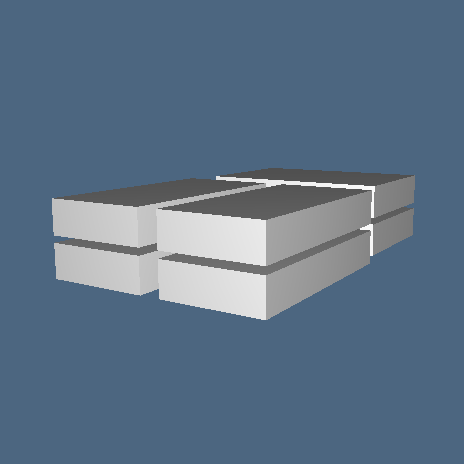
\includegraphics[width=.48\columnwidth]{immagini/test01_1}} \quad 
  %\subfloat[][PF2]
  {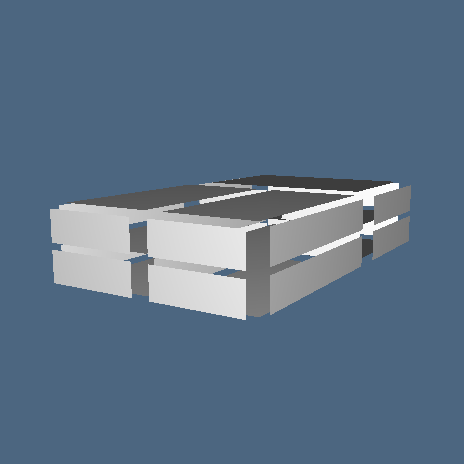
\includegraphics[width=.48\columnwidth]{immagini/test01_2}} \\
  \vspace{0.5 cm}
  %\subfloat[][PF3]
  {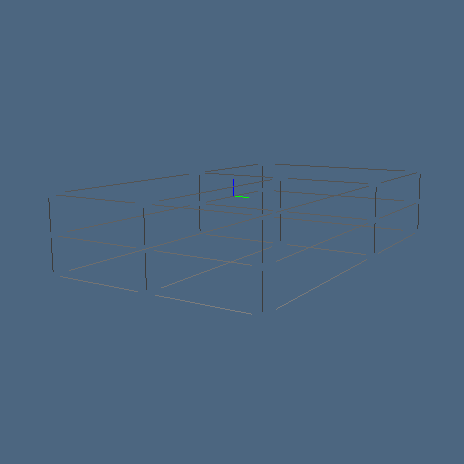
\includegraphics[width=.48\columnwidth]{immagini/test01_3}} \quad
  %\subfloat[][PF4]
  {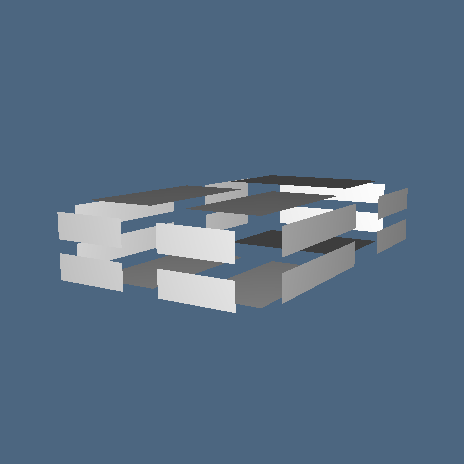
\includegraphics[width=.48\columnwidth]{immagini/test01_4}} \\
  \caption{Risultati grafici durante l'esecuzione di \texttt{test01.jl}}
\label{fig:subfig}
\end{figure}


\subsection{test11}

\noindent \textbf{Python}

\begin{codice}
""" Example of oriented edge drawing """
from larlib import *

V = [[9,0],[13,2],[15,4],[17,8],[14,9],[13,10],[11,11],[9,10],[7,9],[5,9],[3,
8],[0,6],[2,3],[2,1],[5,0],[7,1],[4,2],[12,10],[6,3],[8,3],[3,5],[5,5],[7,6],
[8,5],[10,5],[11,4],[10,2],[13,4],[14,6],[13,7],[11,9],[9,7],[7,7],[4,7],[2,
6],[12,7],[12,5]]

FV = [[0,1,26],[5,6,17],[6,7,17,30],[7,30,31],[7,8,31,32],[24,30,31,35],[3,4,
28],[4,5,17,29,30,35],[4,28,29],[28,29,35,36],[8,9,32,33],[9,10,33],[11,10,
33,34],[11,20,34],[20,33,34],[20,21,32,33],[18,21,22],[21,22,32],[22,23,31,
32],[23,24,31],[11,12,20],[12,16,18,20,21],[18,22,23],[18,19,23],[19,23,24],
[15,19,24,26],[0,15,26],[24,25,26],[24,25,35,36],[2,3,28],[1,2,27,28],[12,13,
16],[13,14,16],[14,15,16,18,19],[1,25,26,27],[25,27,36],[36,27,28]]

VIEW(EXPLODE(1.2,1.2,1)(MKPOLS((V,FV))))
VV = AA(LIST)(range(len(V)))
_,EV = larFacets((V,FV+[range(16)]),dim=2,emptyCellNumber=1)

submodel = mkSignedEdges((V,EV))
VIEW(submodel)
VIEW(larModelNumbering(scalx=1,scaly=1,scalz=1)(V,[VV,EV,FV],submodel,2))
\end{codice}

\vspace{0.5cm}

\noindent \textbf{Julia}

\begin{codice}
using PyCall
using DataStructures

@pyimport larlib as l
@pyimport numpy as np
@pyimport pyplasm as p
@pyimport scipy.sparse as ss
@pyimport sys

include("traduzione.jl")
include("largrid.jl")

V = [[9,0],[13,2],[15,4],[17,8],[14,9],[13,10],[11,11],[9,10],[7,9],[5,9],[3,
8],[0,6],[2,3],[2,1],[5,0],[7,1],[4,2],[12,10],[6,3],[8,3],[3,5],[5,5],[7,6],
[8,5],[10,5],[11,4],[10,2],[13,4],[14,6],[13,7],[11,9],[9,7],[7,7],[4,7],[2,
6],[12,7],[12,5]]

FV = [[0,1,26],[5,6,17],[6,7,17,30],[7,30,31],[7,8,31,32],[24,30,31,35],[3,4,
28],[4,5,17,29,30,35],[4,28,29],[28,29,35,36],[8,9,32,33],[9,10,33],[11,10,
33,34],[11,20,34],[20,33,34],[20,21,32,33],[18,21,22],[21,22,32],[22,23,31,
32],[23,24,31],[11,12,20],[12,16,18,20,21],[18,22,23],[18,19,23],[19,23,24],
[15,19,24,26],[0,15,26],[24,25,26],[24,25,35,36],[2,3,28],[1,2,27,28],[12,13,
16],[13,14,16],[14,15,16,18,19],[1,25,26,27],[25,27,36],[36,27,28]]

larExplodedView(V,FV)
VV = [] 
for i in collect(0:length(V)-1)
    VV = vcat(VV, [[i]])
end 
model = (V, vcat(FV,[collect(0:15)]))
_,EV = plarFacets(model,2,1)

submodel = pmkSignedEdges((V,EV))
p.VIEW(submodel)
\end{codice}

\vspace{0.5 cm}

\begin{figure}[H]
  \centering
  %\subfloat[][PF1]
  {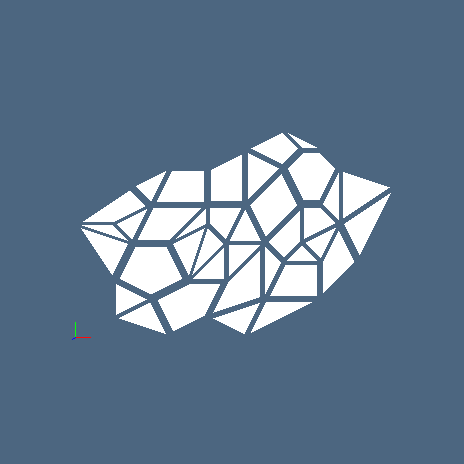
\includegraphics[width=.48\columnwidth]{immagini/test11_1}} \quad 
  %\subfloat[][PF2]
  {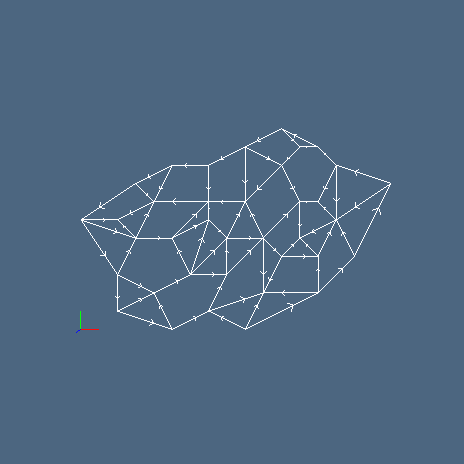
\includegraphics[width=.48\columnwidth]{immagini/test11_2}} \\
  \vspace{0.5 cm}
  %\subfloat[][PF3]
  {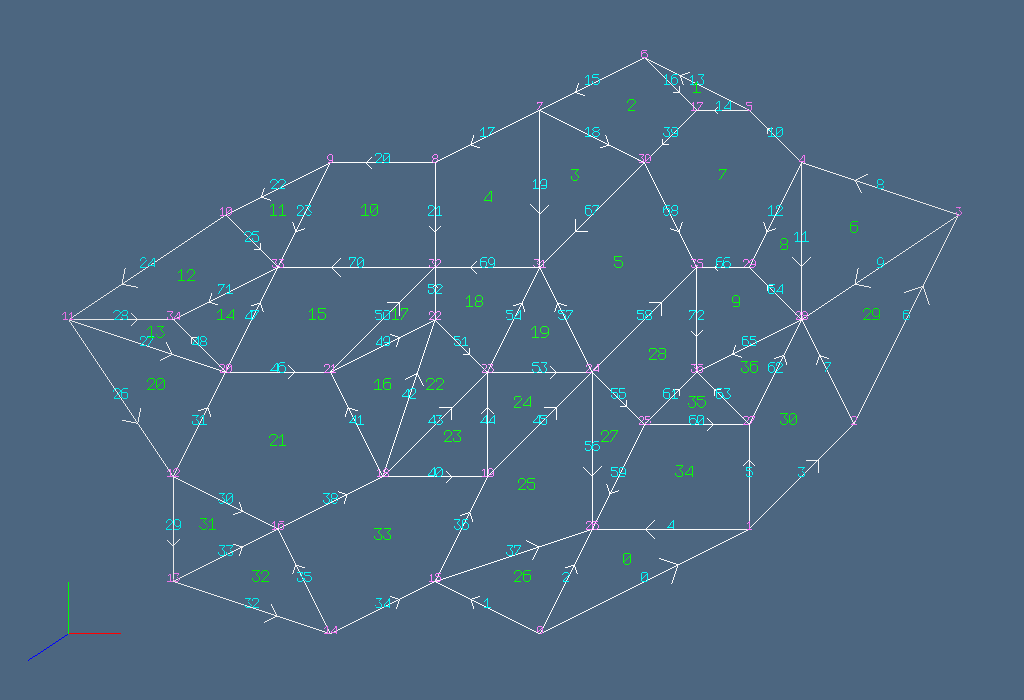
\includegraphics[width=1\columnwidth]{immagini/test11_3b}} \\
  \caption{Risultati grafici durante l'esecuzione di \texttt{test11.jl}}
\label{fig:subfig}
\end{figure}
\singlespacing

\chapter{Conclusioni}

Dallo svolgimento di diversi test sul numero di processori, si nota che la parallelizzazione di alcune delle funzioni rallenta l'esecuzione delle 
stesse. Un altro tentativo � stato effettuato andando ad agire su diversi input di grandi dimensioni. Sono state pertanto confrontate le performance 
delle funzioni parallelizzate con quelle seriali, utilizzando 15 processori, su diversi input di grandi dimensioni. \\

\noindent Segue lo studio sulla funzione \texttt{csrCreate} con diversi input con n = 15. \\

\begin{codice}
input1 = vcat([EV*j for j=1:100]...) 
input2 = vcat([EV*j for j=1:1000]...)
input3 = vcat([EV*j for j=1:5000]...)
\end{codice}

\noindent dove 

\begin{codice}
EV = [[0,1],[0,3],[1,2],[1,3],[1,4],[2,4],[2,5],[3,4],[4,5]] 
\end{codice}

\vspace{0.5 cm}

\noindent \textbf{Tempi della versione seriale}
\begin{codice}
timeinput1 = 0.002113414
timeinput2 = 0.008444055
timeinput3 = 0.050567467
\end{codice}

\vspace{0.5 cm}

\noindent \textbf{Tempi della versione parallela}
\begin{codice}
timepinput1 = 0.002388622
timepinput2 = 0.00893245
timepinput3 = 0.060305142
\end{codice}

\vspace{0.5 cm}

\noindent \textbf{Confronti tra la versione seriale e la parallela tramite il rapporto tra i loro tempi}
\begin{codice}
timeinput1/timepinput1 = 0.8847837790994139
timeinput2/timepinput2 = 0.945323511466619
timeinput3/timepinput3 = 0.8385266218260459
\end{codice}

\vspace{0.5 cm}

\noindent Come si evince dall'esempio di cui sopra, la versione parallela non � efficiente. \\\\

\noindent Esempio sicuramente pi� significativo � dato dallo studio sulla funzione \texttt{csr2DenseMatrix}. \\

\begin{codice}
input1 = vcat([EV*j for j=1:100]...)
input2 = vcat([EV*j for j=1:1000]...)
input3 = vcat([EV*j for j=1:5000]...)
\end{codice}

\vspace{0.5 cm}

\noindent \textbf{Tempi della versione seriale}
\begin{codice}
timeinput1 = 0.009490412
timeinput2 = 0.466812199
timeinput3 = 12.684459215
\end{codice}

\vspace{0.5 cm}

\noindent \textbf{Tempi della versione parallela}
\begin{codice}
timepinput1 = 0.010543615
timepinput2 = 0.669056614
timepinput3 = 14.3567615
\end{codice}

\vspace{0.5 cm}

\noindent \textbf{Confronti tra la versione seriale e la parallela tramite il rapporto tra i loro tempi}
\begin{codice}
timeinput1/timepinput1 = 0.9001098769255138
timeinput2/timepinput2 = 0.6977170380382787
timeinput3/timepinput3 = 0.8835181398674068	
\end{codice}

\vspace{0.5 cm}

\noindent Si pu� dunque concludere che la versione seriale, in caso di grandi input, aiuta a velocizzare il processo.

\end{document}
